\chapter{Waveform Communication}
\label{chapter:ContinuousTimeComm}

In Chapter~\ref{chapter:DiscreteTimeComm}, we introduced digital communication using a discrete-time model that allowed us to ignore the details of the more realistic continuous-time model.
The goal of this chapter is to delve into the details of waveform-based communication and see that the discrete-time model can be derived from the continuous-time model under some conditions.
The \defn{communication}{waveform channel} defines the probabilistic mapping between the deterministic channel input waveform $s(t)$ and the random-process $R(t)$ observed at the output of the channel.
The basic model is that $R(t) = s(t) + N(t)$, where $N(t)$ is Gaussian white-noise random process with autocorrelation function $R_N (\tau) = \delta(\tau) N_0 / 2$.
In some cases, the channel will also act as a linear filter and produce $R(t) = h(t) * s(t) + N(t)$, where $h(t)$ is the channel response.

\begin{figure}
\begin{center}
\begin{psfrags}
\psfrag{c}[c]{Channel}
\psfrag{x}[l]{$s(t)$}
\psfrag{n}[l]{$N(t)$}
\psfrag{r}[l]{$R(t)$}
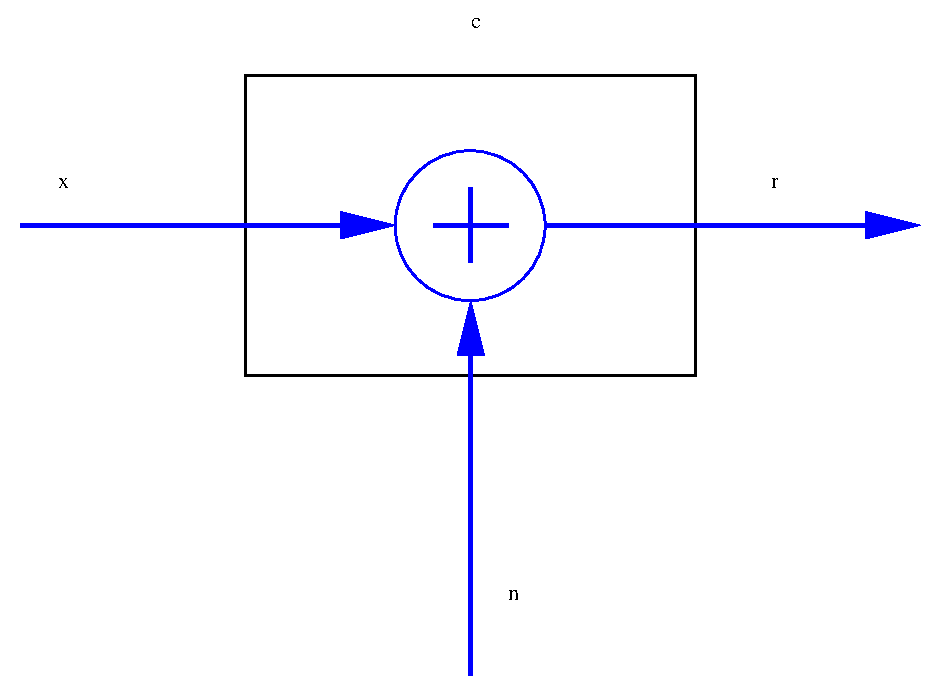
\epsfig{file=Figures/channel.eps,width=6.5cm}
\end{psfrags}
\end{center}
\caption{Block diagram of a basic waveform channel for input signal $s(t)$, noise process $N(t)$, and received signal $R(t)$.}
\end{figure}

\iffalse
\emph{Modulation} is the process by which a string of bits is converted into a signal suitable for transmission over a communication channel.
\emph{Demodulation} is the reverse operation at the destination where the information symbols are extracted from the received signal.
The shapes of the waveforms employed to create the transmitted signal are critical to the overall performance and operation of the system.
In many implementations, a high-frequency sinusoid is used, in addition to baseband pulse waveforms, as carrier to center the baseband signal at its intended frequency.
We initiate our study of modulation and demodulation with baseband signals; advanced considerations associated with carrier sinusoids and bandpass processes will be explored later.

Let $\{ s_k \in \{ 0, 1 \}^b \}$ be a sequence of binary symbols to be transmitted to a destination, and let $f : \{ 0, 1 \}^b \mapsto \mathbb{R}$ be an invertible function that takes a string of $b$ bits as input, and gives a real number as output, with $u_k = f(s_k)$.
Suppose further that several distinct waveforms are available at the transmitter, which we denote by $\{ \phi_k (t) \}$.
We study communication systems that modulate binary symbols in two steps.
First, a collection of binary data $\{ s_k \}$ is converted into a string of real numbers $\{ u_k \}$ using function $f(\cdot)$.
Next, these real numbers are used to form a transmission signal by creating a weighted linear combination of the basis functions,
\begin{equation*}
u(t) = \sum_k u_k \phi_k(t) .
\end{equation*}
This procedure provides a simple framework to transition back and forth between a digital sequence and the corresponding modulated signal.
At the destination, the sequence of binary symbols is demodulated by passing the received signal through linear time-invariant filters, and then mapping the resulting real number to one of the possible $b$-bit messsages.
\fi

\section{A Single Digital Symbol}

Suppose that one would like to send a single digital symbol taking $M$ different values to a receiver through a waveform channel.
Then, one can associate a waveform $s_m (t)$ with each symbol $m=1,\ldots,M$ and transmit the waveform assigned with the desired message.
For mathematical convenience, we assume that each waveform is zero outside of the interval $0\leq t\leq T$ where $T$ is symbol duration.

The demodulation process is based on mathematical operation, known as an inner product, that maps any two signals to a complex number.
The \defn{communication}{inner product} $\langle s(t) , r(t) \rangle$ between the signals $s(t)$ and $r(t)$ is defined by
\begin{equation*}
\left\langle s (t), r^* (t) \right\rangle
= \int_{-\infty}^{\infty} s(t) r^* (t) dt,
\end{equation*}
where $r^* (t)$ is the complex conjugate of $r(t)$.
Mathematically, we are treating the set of all finite-energy signals as a \defn{communication}{vector space} and using this inner product to define distances and angles in this space.
The energy (or length squared) of a signal $s(t)$ is given by
\[ \int_{-\infty}^{\infty} \left| s(t) \right|^2 dt = \langle s(t),s(t) \rangle. \]
Two signals $s_1 (t),s_2 (t)$ are said to be \defn{communication}{orthogonal} if $\langle s_1(t),s_2 (t)\rangle = 0$.
A signal $s(t)$ is said to be \textbf{normalized} if $\langle s(t),s(t) \rangle = 1$.
A set of signals is said to be \textbf{orthonormal} if every signal in the set is orthogonal to every other signal in the set and all signals in the set are normalized.
The set of all linear combinations of signal waveforms is called the \defn{communication}{signal space}.

\subsubsection{Orthonormal Waveforms}
The simplest scenario occurs when the set of signal waveforms $\{ s_1 (t), \ldots , s_M (t) \}$ is orthonormal.
In this case, one can demodulate the received signal $R(t)$ by computing
\[ R_j = \langle R(t), s_j (t) \rangle, \]
for each $j=1,\ldots,M$.
Due to the noise process, the resulting values $R_1 , \ldots, R_M$ are Gaussian random variables.
Their expected values depend on which waveform was actually transmitted.
If $s_m (t)$ was transmitted, then $R(t) = s_m(t) + N(t)$, $E[R(t)] = s_m(t)$, and we have
\begin{align*}
E \left[R_j \right]
&= E \left[ \int_{-\infty}^{\infty} R(t) s_j^* (t) dt \right] \\
&= \int_{-\infty}^{\infty} E \left[ R(t) \right] s_j^* (t) dt \\
&= \int_{-\infty}^{\infty} s_m (t) s_j^* (t) dt \\
&= \delta_{m,j}.
\end{align*}

The random variables $R_1, \ldots , R_M$ also have some other nice properties.
They are uncorrelated because the the waveforms are orthogonal and they have variance $N_0  / 2$ because the waveforms are normalized.
Proving this statement will be left as a homework exercise.

This transforms the waveform detection problem into a detection problem for a length-$M$ vector of Gaussian random variables.
If $s_m (t)$ was transmitted, then the mean of the random vector is the unit vector with a one in the $m$th position.
Based on the techniques from Chapter~\ref{chapter:DiscreteTimeComm}, the maximum-likelihood decision rule chooses the symbol whose unit vector is closest to the random vector $R_1,\ldots,R_M$ in Euclidean distance.

\begin{example}[Frequency-Shift Keying] \label{example:TSpacedTruncatedSinusoids}
For a fixed time-interval $T$, consider the collection of waveforms given by
\begin{equation*}
s_m(t) = \frac{1}{\sqrt{T}} e^{2 \pi i \frac{m}{T} t} \mathrm{rect} \left( \frac{t}{T} \right) .
\end{equation*}
for $m = 1, \ldots, M$.
This set of waveforms is known as $M$-ary frequency-shift keying (or $M$-FSK).
We wish to show that these waveforms are orthonormal.

To prove that they are orthogonal, we consider the inner product of $s_m(t)$ and $s_n(t)$ when $m \neq n$,
\begin{equation*}
\begin{split}
\left\langle s_m (t), s_n (t) \right\rangle
&= \int_{\mathbb{R}} s_m (t) s_n^* (t) dt 
= \frac{1}{T} \int_{-\frac{T}{2}}^{\frac{T}{2}}
e^{2 \pi i \frac{m}{T} t} e^{- 2 \pi i \frac{n}{T} t} dt \\
&= \frac{1}{T} \int_{-\frac{T}{2}}^{\frac{T}{2}}
e^{2 \pi i \frac{(m-n)}{T} t} dt
= 0 .
\end{split}
\end{equation*}
Next, we show that these basis elements have unit energy,
\begin{equation*}
\begin{split}
\left\| s_m(t) \right\|^2
&= \int_{\mathbb{R}} s_m (t) s_m^* (t) dt 
= \frac{1}{T} \int_{-\frac{T}{2}}^{\frac{T}{2}}
e^{2 \pi i \frac{m}{T} t} e^{- 2 \pi i \frac{m}{T} t} dt \\
&= \frac{1}{T} \int_{-\frac{T}{2}}^{\frac{T}{2}} dt
= 1 .
\end{split}
\end{equation*}
\end{example}

\subsubsection{General Waveforms}

When the signal waveforms are not orthonormal, the detection problem is solved most easily by constructing a set of orthonormal basis vectors for the signal space.
In general, this can be accomplished by applying the Gram-Schmidt orthogonalization process to the signal waveforms.
Rather than focusing on this process, we assume that $\{ \phi_1 (t), \ldots , \phi_N (t) \}$ is an orthonormal set of waveforms such that the coefficients $a_{m,k}$ allow us to write
\[ s_m (t) = \sum_{k=1}^N a_{m,k} \phi_k (t). \]
This implies that the orthonormal set spans the signal space.

In this case, the received signal $R(t)$ can be demodulated by computing
\[ R_j = \langle R(t), \phi_j (t) \rangle, \]
for each $j=1,\ldots,N$.
Again, the noise process implies that $R_1 , \ldots, R_N$ are Gaussian random variables whose means are determined by which waveform was actually transmitted.
For $j=1,\ldots,N$, the noise component of $R_j$ is independent of the transmitted signal, and is given by
\[ N_j = \int_{-\infty}^{\infty} N(t) \phi_j^* dt. \]
Therefore, $R_j = E[R_j] + N_j$ and the mean, if $s_m (t)$ was transmitted, is given by
\begin{align*}
E \left[R_j \right]
&= E \left[ \int_{-\infty}^{\infty} R(t) \phi_j^* (t) dt \right] \\
&= \int_{-\infty}^{\infty} E \left[ R(t) \right] \phi_j^* (t) dt \\
&= \int_{-\infty}^{\infty} s_m (t) \phi_j^* (t) dt \\
&= \int_{-\infty}^{\infty} \left( \sum_{k=1}^N a_{m,k} \phi_k (t) \right) \phi_j^* (t) dt \\
&= \sum_{k=1}^N a_{m,k} \delta_{k,j} dt \\
&= a_{m,j}. \\
\end{align*}

Again, we have transformed the waveform detection problem into a detection problem for a vector of Gaussian random variables.
In this case, however, there are $M$ different mean vectors of dimension $N$.
Based on the techniques from Chapter~\ref{chapter:DiscreteTimeComm}, the maximum-likelihood decision rule chooses the symbol $\hat{m}$ whose coordinate vector $(a_{\hat{m},1},\ldots. a_{\hat{m},N})$ is closest to the random vector $R_1,\ldots,R_N$ in Euclidean distance.

This approach can be seen as first projecting the infinite-dimensional received waveform onto a finite-dimensional subspace and then using the optimal detector on this finite-dimensional space.
To show that this overall approach is optimal, one must also prove that the residual waveform
\[ \tilde{N}(t) = R(t) - \sum_{j=1}^N R_j \phi_j (t) \]
does not contain any information relevant to the decision.
While this is indeed true, we ignore this detail for now.

\begin{figure}
\begin{center}
\begin{psfrags}
\psfrag{p1}[l]{$\phi_1(t)$}
\psfrag{p2}[l]{$\phi_2(t)$}
\psfrag{p3}[l]{$\phi_{N-1}(t)$}
\psfrag{p4}[l]{$\phi_N(t)$}
\psfrag{i}[c]{$\int_{0}^T (\cdot) dt$}
\psfrag{r}[l]{$r(t)$}
\psfrag{r1}[l]{$r_1$}
\psfrag{r2}[l]{$r_2$}
\psfrag{r3}[l]{$r_{N-1}$}
\psfrag{r4}[l]{$r_N$}
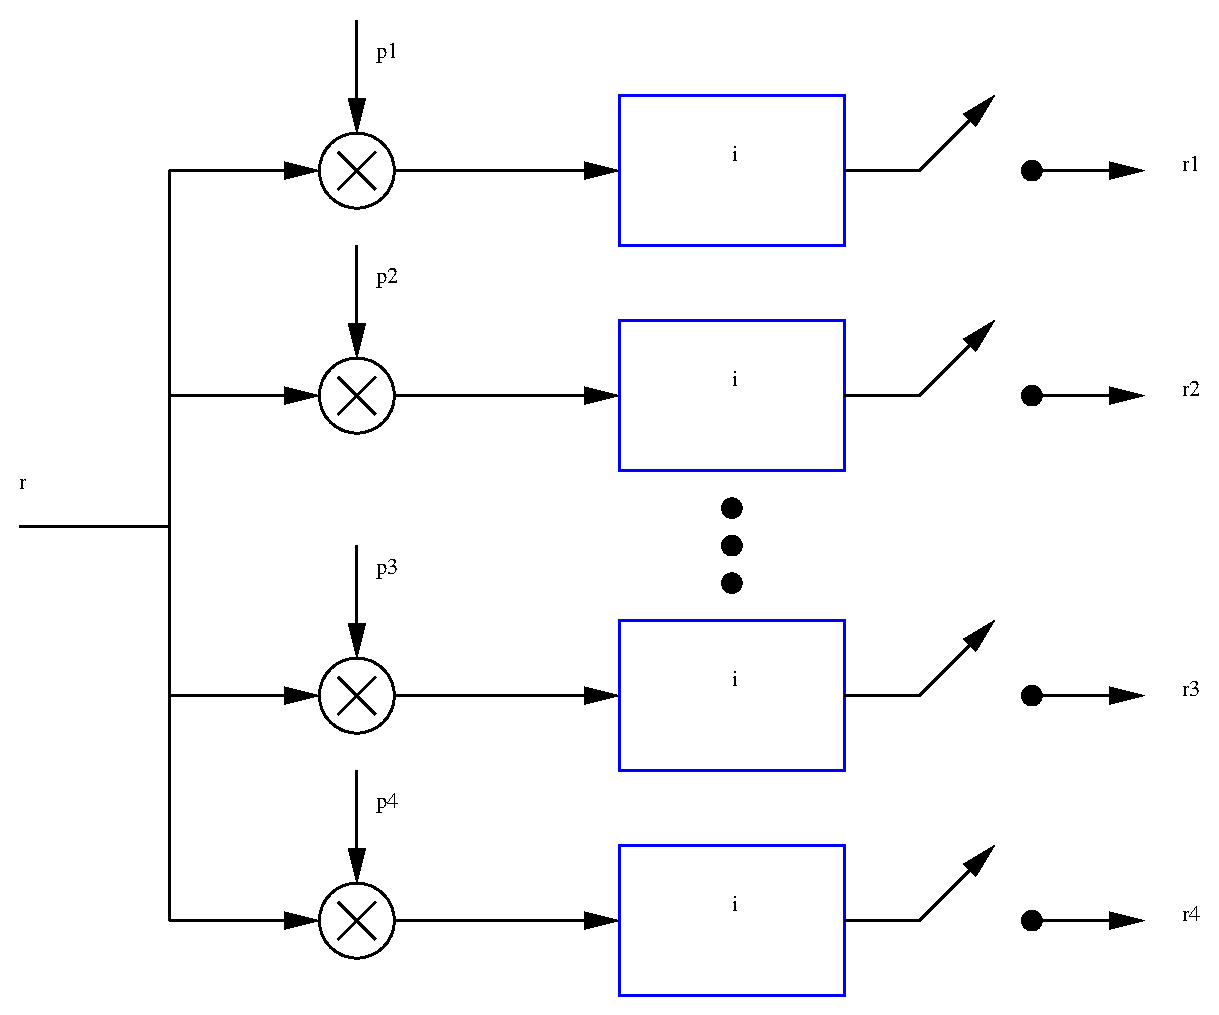
\epsfig{file=Figures/correlator.eps,width=8cm}
\end{psfrags}
\end{center}
\caption{For a particular realization $r(t)$ of the received signal, the received projection onto the signal-space basis vector can be computed by a bank of correlators.}
\end{figure}

\iffalse
The $T$-spaced truncated sinusoids of Example~\ref{example:TSpacedTruncatedSinusoids} form a collection of basis waveforms that can be employed to create a signal.
To further illustrate this point, we show explicitly how orthonormal waveforms can be used in the modulation and demodulation of data symbols.
Suppose that a signal is produced by taking a linear combination of the waveforms $\{ \phi_k(t) \}$, weighted by the real numbers $\{ u_k \}$, with
\begin{equation*}
u(t) = \sum_{k} u_k \phi_k(t) .
\end{equation*}
In the absence of noise, the original sequence of real numbers can be recovered at the destination using the projections afforded by the basis elements $\{ \phi_k (t) \}$.
In particular, we have
\begin{equation*}
\begin{split}
\left\langle u(t), \phi_n(t) \right\rangle
&= \int_{\mathbb{R}}
\left( \sum_{m=1}^M u_m \phi_m(t) \right) \phi_n^*(t) dt \\
&= \sum_{m=1}^M u_m \int_{\mathbb{R}}
\phi_m(t) \phi_n^*(t) dt
= u_n .
\end{split}
\end{equation*}

\begin{example}[Binary Modulation]
In this example, we consider the simplest possible scenario, the modulation of a single bit.
Suppose that a bit $s$ is mapped into the real numbers according to the rule
\begin{equation*}
u = f(s) = \begin{cases} -A, & s = 0 \\
A, & s = 1 , \end{cases}
\end{equation*}
where $A$ is a positive number and represents the amplitude of the waveform.
Then, the transmitted signal becomes
\begin{equation*}
u(t) = u \phi (t) .
\end{equation*}
To extract the value of $u$ for the signal $u(t)$, we simply compute the inner product of the signal with the basis element $\phi(t)$, which yields $u = \langle u(t), \phi(t) \rangle$.
The original bit $s$ is then obtained by taking the inverse of $u$ under function $f(\cdot)$, with $s = f^{-1} (u)$.
\end{example}

Except for noise considerations, this section presents the first principles under which modern digital communication systems operate.
Below, we continue our analysis of modulation and demodulation schemes by looking at the implications of sending multiple waveforms over time.
\fi

\section{Time-Shift Waveforms}

In practical communication systems, a succession of symbols is transmitted to the destination.
Not only can waveforms interfere with one another in signal space, they can also disrupt signal quality across time.
Suppose that a different symbol is sent every $T$ seconds using time shifts of a basic pulse waveform $p(t)$.
The transmitted signal, accounting for the different values of $\{ u_n \}$, is equal to
\begin{equation*}
u(t) = \sum_{n} u_n p (t - nT) .
\end{equation*}
Note that in this case, the available waveforms are simply translated versions of one another.
Ideally, we want the collection $\{ p(t - nT) \}$ to be orthonormal.
This would greatly simplify system implementation and decision making at the receiver.
However, we cannot use standard techniques such as the Gram-Schmidt procedure to construct a set of orthogonal waveforms, because the elements of $\{ p(t - nT) \}$ are constrained to be translated version of one another.
Getting an orthonormal set requires more work.

As before, each symbol $u_n$ is identified at the destination by passing the received signal through a linear time-invariant filter, which is mathematically equivalent to performing an inner-product integral.
Since the waveforms $\{ p(t-nT) \}$ are shifted versions of a same function, it is natural to expect the various filters to implement projections onto shifted versions of a single element $q(t)$.
A uniform treatment of the demodulation operation can therefore be conducted by looking a the inner product between $u(t)$ and $q(t-\tau)$.
Let
\begin{equation} \label{equation:InnerProductReceiver}
\begin{split}
r(\tau) &= \langle u(t), q(t-\tau) \rangle
= \int_{\mathbb{R}} u(t) q^*(t-\tau) dt \\
&= \sum_{k} u_k \int_{\mathbb{R}} p(t - kT) q^*(t-\tau) dt \\
&= \sum_{k} u_k g(\tau - kT) .
\end{split}
\end{equation}
where $g(\tau) = \langle p(t), q(t-\tau) \rangle$.
By convention, $q(t)$ is defined such that element $u_n$ is acquired by looking at $r(nT)$.
Rewritting \eqref{equation:InnerProductReceiver}, we get
\begin{equation*}
r(nT) = u_n g(0) + \sum_{k \neq n} u_k g((n - k)T) .
\end{equation*}
The first term in this expansion contains the desired symbols.
The remaining sum is called \emph{intersymbol interference (ISI)}; it contains the contributions from all the other time-shifted waveforms.
To retrieve the information sequence unambiguously, we wish to have $r(nT) = u_n$, irrespective of the values in the sequence $\{ u_k \}$.
This will be achieved provided that
\begin{equation} \label{equation:NoInterSymbolInterferenceSpecification}
g(nT) = \begin{cases} 1, & k = n \\
0, & \text{otherwise} . \end{cases}
\end{equation}
To understand how this condition impacts our choice of a functions $p(t)$ and $q(t)$, we use the frequency representation of $g(\tau)$.
Looking at the inverse Fourier transform of $\hat{g}(f)$, we get
\begin{equation*}
\begin{split}
g(\tau) &= \mathcal{F}^{-1} \left[ \hat{g} (f) \right]
= \int_{\mathbb{R}} \hat{g}(f) e^{2 \pi i f \tau} df \\
&= \sum_{m = -\infty}^{\infty} \int_{-\frac{F}{2}}^{\frac{F}{2}}
\hat{g} (f - Fm) e^{2 \pi i (f - mF) \tau} df
\end{split}
\end{equation*}
where, for reasons that will soon be obvious, we have judiciously selected $F = \frac{1}{T}$.
The value of $g(\tau)$ at the sample points $\{ \tau = nT : n \in \mathbb{Z} \}$ can then be expressed as
\begin{equation} \label{equation:SamplePointsNoISI}
\begin{split}
g(nT) &= \sum_{m = -\infty}^{\infty} \int_{-\frac{F}{2}}^{\frac{F}{2}}
\hat{g} \left( f - \frac{m}{T} \right) e^{2 \pi i \left( f - \frac{m}{T} \right) nT} df \\
&= \int_{-\frac{F}{2}}^{\frac{F}{2}}
\left( \sum_{m = -\infty}^{\infty} \hat{g} \left( f - \frac{m}{T} \right) \right)
e^{2 \pi i n T f} df \\
&= \frac{1}{F} \int_{-\frac{F}{2}}^{\frac{F}{2}}
\hat{z} (f) e^{2 \pi i \frac{n}{F} f} df ,
\end{split}
\end{equation}
where we have defined
\begin{equation*}
\hat{z}(f) = F \sum_{m = -\infty}^{\infty} \hat{g} \left( f - \frac{m}{T} \right)
\mathrm{rect} \left( \frac{f}{F} \right) .
\end{equation*}
Notice the similarity between \eqref{equation:SamplePointsNoISI} and the Fourier series representation of a time-limited function.
Specifically, $\{ g(nT) : n \in \mathbb{Z} \}$ can be viewed as the Fourier series coefficients of the frequency-limited function $\hat{z}(f)$.
Under condition \eqref{equation:NoInterSymbolInterferenceSpecification}, and using the reconstruction formula for Fourier series, we get
\begin{equation} \label{equation:NoInterSymbolInterference}
\hat{z}(f) = \sum_{n = -\infty}^{\infty} g(nT) e^{2 \pi i \frac{n}{F} f}
\mathrm{rect} \left( \frac{f}{F} \right)
= \mathrm{rect} \left( \frac{f}{F} \right)
\end{equation}
because $g(nT) = 0$ whenever $n \neq 0$.
Thus, the system exhibits no intersymbol interference if and only if \eqref{equation:NoInterSymbolInterference} holds.

Equivalently, condition~\eqref{equation:NoInterSymbolInterferenceSpecification} is satisfied whenever
\begin{equation} \label{equation:NyquistNoISI}
\sum_{m = -\infty}^{\infty} \hat{g} \left( f - \frac{m}{T} \right) = T .
\end{equation}
We formalize this key result, known as the \emph{Nyquist pulse-shaping criterion}, in the theorem below.

\begin{theorem}[Nyquist] \label{theorem:NyquistPulseCriterion}
Let $g(\tau)$ and $\hat{g}(f)$ be square integrable functions that are Fourier transforms of each other.
Furthermore, assume that the function
\begin{equation*}
\hat{z} (f) = F \sum_{m=-\infty}^{\infty} \hat{g} \left( f - \frac{m}{T} \right)
\mathrm{rect} (fT)
\end{equation*}
has finite energy.
Then, a necessary and sufficient condition for
\begin{equation*}
g(nT) = \begin{cases} 1, & n = 0 \\
0, & \text{otherwise} \end{cases}
\end{equation*}
is that the following equality holds for all values of $f \in \mathbb{R}$,
\begin{equation} \label{equation:NyquistCriterionFrequencyCondition}
\sum_{m=-\infty}^{\infty} \hat{g} \left( f - \frac{m}{T} \right) = T .
\end{equation}
\end{theorem}

\begin{example}
One of the simplest possible choices for waveforms $p(t)$ and $q(t)$ is
\begin{equation*}
p(t) = q(t) = \frac{1}{\sqrt{T}} \mathrm{rect} \left( \frac{t}{T} \right) .
\end{equation*}
In this case, we get
\begin{equation*}
\begin{split}
g(\tau) &= \langle p(t), q(t-\tau) \rangle
= \frac{1}{T} \int_{\mathbb{R}} \mathrm{rect} \left( \frac{t}{T} \right)
\mathrm{rect} \left( \frac{t - \tau}{T} \right) dt \\
&= \frac{1}{T} \int_{\mathbb{R}} \mathrm{rect} \left( \frac{t}{T} \right)
\mathrm{rect} \left( \frac{\tau - t}{T} \right) dt
= \frac{1}{T} \mathrm{rect} \left( \frac{t}{T} \right)
\ast \mathrm{rect}\left( \frac{t}{T} \right) .
\end{split}
\end{equation*}
Obviously, this selection leads to the desired property with $g(0) = 1$, and $g(nT) = 0$ for any non-zero integer~$n$.
One of the design issues with the rectangular pulse is that its bandwidth is infinite and decays slowly.
This becomes a problem in most practical systems where spectral bandwidth comes at a premium.
\end{example}

\begin{example}
Consider the pulse-shaping criterion applied to
\begin{equation*}
p(t) = q(t) = \frac{1}{\sqrt{T}} \mathrm{sinc} \left( \frac{t}{T} \right) .
\end{equation*}
We wish to show that this choice of waveforms satisfies the Nyquist criterion and leads to a set of orthogonal time-shift waveforms.

First, we find an expression for $g(\tau)$,
\begin{equation*}
\begin{split}
g(\tau) &= \langle p(t), q(t-\tau) \rangle
= \frac{1}{T} \int_{\mathbb{R}} \mathrm{sinc} \left( \frac{t}{T} \right)
\mathrm{sinc} \left( \frac{t - \tau}{T} \right) dt \\
&= \frac{1}{T} \int_{\mathbb{R}} \mathrm{sinc} \left( \frac{t}{T} \right)
\mathrm{sinc} \left( \frac{\tau - t}{T} \right) dt
= \frac{1}{T} \mathrm{sinc} \left( \frac{t}{T} \right)
\ast \mathrm{sinc} \left( \frac{t}{T} \right) .
\end{split}
\end{equation*}
In the frequency domain, we have
\begin{equation*}
\begin{split}
\hat{g}(f) &= \mathcal{F} \left[ g(\tau) \right]
= \frac{1}{T} \mathcal{F} \left[ \mathrm{sinc} \left( \frac{t}{T} \right) \right]
\mathcal{F} \left[ \mathrm{sinc} \left( \frac{t}{T} \right) \right] \\
&= T \mathrm{rect} (T f) \mathrm{rect} (T f)
= T \mathrm{rect} (T f) .
\end{split}
\end{equation*}
We can therefore verify condition~\eqref{equation:NyquistCriterionFrequencyCondition} as
\begin{equation*}
\sum_{m = -\infty}^{\infty}
\hat{g} \left( f - \frac{m}{T} \right)
= \sum_{m = - \infty}^{\infty} T \mathrm{rect} (Tf - m)
= T .
\end{equation*}
That is, the conditions of Theorem~\ref{theorem:NyquistPulseCriterion} hold and, consequently, $g(0) = 1$ and $g(n) = 0$ for any non-zero integer.
One of the positive attributes of the $\mathrm{sinc} (\cdot)$ waveform is that it is bandwidth-limited.
However, this pulse is not time-limited and it is therefore somewhat impractical, as using $\mathrm{sinc} (\cdot)$ waveforms would entail infinite delay at the destination.
\end{example}

Although, there are many choices for $\hat{g}(f)$ that satisfy Theorem~\ref{theorem:NyquistPulseCriterion}, we are primarily interested in waveforms that are approximately both bandwidth-limited and time-limited.
The \emph{Nyquist bandwidth} associated with a signal
\begin{equation*}
u(t) = \sum_k u_k p(t -kT)
\end{equation*}
is defined by $\frac{1}{2T}$; it represents the smallest possible bandwidth for which it is possible to prevent intersymbol interference.
The spectral bandwidth of $\hat{g}(f)$ is the smallest possible value of $W$ such that $\hat{g}(f) = 0$ for $|f| > W$.

\iffalse
\subsection{Pulse Amplitude Modulation}

Pulse amplitude modulation (PAM) is a simple form of modulation, where data is embedded in the amplitude of a single waveform,
\begin{equation*}
u(t) = u \phi (t) .
\end{equation*}
The incoming binary data is segmented into binary symbols of $b$ bits, and each block is mapped into one of $2^b = M$ possible real numbers within the constellation set $\mathcal{A} = \{ a_1, \ldots, a_M \}$.
In the absence of noise and interference, the value of the sent $b$-bit message is recovered by first taking the inner product of $u(t)$ with the basis element $\phi (t)$,
\begin{equation*}
u = \langle u(t), \phi(t) \rangle = \int_{\mathbb{R}} u(t) \phi^*(t) dt ,
\end{equation*}
and then extracting the original $b$ bits from $u$, using the inverse map.
In standard $M$-PAM, where $M = 2^b$, the amplitude set is equal to
\begin{equation*}
\mathcal{A} = \left\{ - \frac{d(M-1)}{2} , \ldots, - \frac{d}{2}, \frac{d}{2}, \ldots, \frac{d(M-1)}{2} \right\} ,
\end{equation*}
and $d$ denotes the distance between adjacent points.

\subsection{Quadrature Amplitude Modulation}

A closely related modulation scheme is quadrature amplitude modulation (QAM).
In this scheme, data is conveyed to the destination by changing the amplitude of two carrier waves.
Equivalently, QAM can be interpreted as modulating a compex amplitude onto a single waveform,
\begin{equation*}
u(t) = (u + iv) \phi(t) .
\end{equation*}
In both cases, the space spanned by $u(t)$ is two-dimensional (over the real numbers), and the constellation can be abstracted to $\mathcal{A} = \{ (a_1, b_1), \ldots, (a_M, b_M) \}$ where $M = 2^b$ as before.
In a noiseless environment, the modulating scalar $u + iv$ can be extracted from $u(t)$ using the inner product
\begin{equation*}
u + i v = \left\langle u(t), \phi(t) \right\rangle .
\end{equation*}
Note that we can write the received signal in vector form as
\begin{equation*}
(u, v) = \left( \Re \left( \left\langle u(t), \phi(t) \right\rangle \right),
\Im \left( \left\langle u(t), \phi(t) \right\rangle \right) \right) .
\end{equation*}
The latter interpretation, where QAM is seen as a single waveform modulated by a complex number, originates from the fact that baseband waveforms are often modulated by sinusoid carriers.
The in-phase ($\cos (2 \pi f_{\mathrm{c}} t)$) and quadrature ($\sin (2 \pi f_{\mathrm{c}} t)$) components of the bandpass signal then correspond to the real and imaginary parts of the baseband waveform.

\begin{example}[Phase Shift Keying]
In phase shift keying (PSK), the transmitted signal $u(t)$ is given by
\begin{equation*}
u(t) = \frac{1}{\sqrt{T}} e^{2 \pi i f_{\mathrm{c}} t + i \theta}
\mathrm{rect} \left( \frac{t}{T} \right) ,
\end{equation*}
where $\theta$ is one of finitely many possibility and the carrier freqency $f_{\mathrm{c}}$ is an integer multiple of $\frac{1}{T}$.
The data in PSK is embedded in $\theta$, the phase of the sinusoid.
Note that the function $u(t)$ can be rewritten as
\begin{equation*}
\begin{split}
u(t) &= e^{i \theta} \frac{1}{\sqrt{T}} e^{i (2 \pi f_{\mathrm{c}} t + \theta)}
= \left( \cos (\theta) + i \sin (\theta) \right) \phi (t) \\
&= (u + iv) \phi (t) .
\end{split}
\end{equation*}
That is, the signal constellation in PSK is constrained to lie on the unit circle.
\end{example}



\newpage

\section{Transmitting symbols over Time}

\subsection{Orthogonality in Time}

\subsection{The Nyquist Criterion}
HERE

\newpage

\section{High-Dimentional Signal Constellations}

\subsection{Orthogonal Signal Waveforms}

\subsection{Simplex Signal Waveforms}

\subsection{Bi-Orthogonal Signal Waveforms}


\section{Signal Space Representation}

Let $\mathcal{W} = \{ \phi_1 (t), \ldots, \phi_D (t) \}$ be an orthonormal set of functions.
Furthermore, suppose that this set possesses the following property,
\begin{equation*}
\left\langle \phi_m \left( t - \frac{k}{T} \right),
\phi_n \left( t - \frac{l}{T} \right) \right\rangle
= \int_{\mathbb{R}} \phi_m \left( t - \frac{k}{T} \right)
\phi_n^* \left( t - \frac{l}{T} \right) dt 
= 0
\end{equation*}
for all $k, l, m, n \in \mathbb{Z}$, except cases where $k = l$ and $m = n$.


\begin{example}[$T$-spaced sinc functions]
This time, let
\begin{equation*}
\phi_m(t) = \frac{1}{\sqrt{T}} e^{-2 \pi i \frac{m}{T} t} \mathrm{sinc} \left( \frac{t}{T} \right)
\end{equation*}
\end{example}



Furthermore, the energy of the transmitted waveform depends on the value of $A$,
\begin{equation*}
\| u(t) \|^2 = \| u_1 \phi_1 (t) \|^2 = |u_1|^2 \| \phi_1(t) \|^2 = A^2 .
\end{equation*}
Naturally, the larger the amplitude is, the greater the energy of the signal becomes.
\section{Detection}

\section{Synchronization}

When the incoming bits are independent, each with equal probabilities of being zero or one, the transmitted waveform becomes a stochastic signal $U(t) = U \phi(t)$.
We can compute the energy of this random waveform $U(t)$ as
\begin{equation*}
\begin{split}
E_{\mathrm{s}} &= \mathrm{E} \left[ \int_{\mathbb{R}} |U(t)|^2 dt \right]
= \mathrm{E} \left[ U^2 \right] \| \phi (t) \|^2 \\
&= \sum_{m=1}^M \frac{1}{M} \frac{(2m - M - 1)^2 d^2}{2} \\
&= \frac{\left( M^2 - 1 \right) d^2}{12} .
\end{split}
\end{equation*}
That is, the average energy used per transmitted symbol is $\frac{(M^2 - 1) d^2}{12}$ and, correspondingly, the average energy per bit is
\begin{equation*}
E_{\mathrm{b}} = \frac{ E_{\mathrm{s}} }{M}
= \frac{\left( M^2 - 1 \right) d^2}{12M}
= \frac{\left( 2^{2b} - 1 \right) d^2}{12 \cdot 2^b} .
\end{equation*}
Roughly speaking, for large PAM constellations, the energy consumption per bit doubles with every additional bit.


\subsection{Linear Time-Invariant Filters and Inner Products}

\fi

